
In the previous section, we defined valuative capacity for a compact subset $S$ of an ultrametric space $(M, \rho)$. We also got a glimpse into the way the valuative capacity of $S$ interacts with its other properties, such as the set of distances occurring in $S$ and the lattice of closed balls in $S$ (or equivalently, if $S$ has enough structure, a lattice of subgroups).\\

In this section, we offer a more detailed study of the interaction between the valuative capacity of $S$ and the lattice of closed balls in $S$. In particular, we  show how, if $S$ is compact and discretely-valued, the lattice of closed balls can be used to compute the first $n$ terms of a $\rho-$ordering of $S$ (for any $n < \infty$). In the following chapter we show how, in some cases, this extends to being able to derive a formula for the valuative capacity of $S$.\\

Similar results have been found for the special case of ultrametric fields in \cite{cef}. We extend these results by moving to a more general setting, showing that much can be said about capacity in $S$ without appealing to any underlying algebraic structure. Significant portions of the theory developed in this chapter was guided by an empirical investigation into the capacity of product spaces, which we describe in the next chapter. The code that performed these calculations is included in the appendix.\\

We assume throughout this section that $S$ is a compact, discretely-valued subset of an ultrametric space $(M, \rho)$.\\

\subsection*{Subspaces of $S$}
In the section we explore the subspaces of $S$ formed by considering closed balls of some fixed radius.  Recall from the previous section that if $S$ is compact and discretely-valued, then the set of distances occurring in $S$ is a discrete, bounded subset of $\mathbb{R}$ and so we may represent the set of distances by a sequence in decreasing order. As before, let the decreasing sequence of distances in $S$ be given by  $\Gamma_S =\{\gamma_0=\text{diam}(S), \gamma_1,\ldots,\gamma_\infty=0\}$.\\

 Now fix some $k \in \mathbb{N}$, and consider for a moment the set of closed balls of radius $\gamma_k$ in $S$. We could denote these alternatively by $B^M(x, \gamma_k) \cap S$ or by  $B^S(x, \gamma_k)$, but when there is no risk of confusion, we will denote them simply by $B(x, \gamma_k)$. Clearly, the set  $\{B(x, \gamma_k); x \in S\}$ forms a cover of $S$. Although we have build the cover using closed balls, since we are in an ultrametric space, this gives an open cover of $S$ (in fact, each element in the cover is not only an open set, but also an open ball for some radius slightly bigger than $\gamma_k$). Then since $S$ is compact, we must have some $x_1,\ldots, x_n$  such that $S= \cup_{i=1}^n B(x_i, \gamma_k)$. In fact,  since $\rho$ is an ultrametric, we can pick the $x_i$'s so that $\cup_{i=1}^n B(x_i, \gamma_k)$ will be a disjoint union and therefore a finite partition of $S$. Note that both $n$ and the $x_i$'s depend on our fixed $k$, but that $n$ is independent of the $x_i$'s, since any choice of centres is equivalent. We rephrase this with following definition and lemma:\\

\begin{definition}
For $S$ and $\Gamma_S$ as above, and $k \in \mathbb{N}$, fixed,  define $\sim_k$ to  be the relation on $S$ given by \[x \sim_k y\text{ if and only if  }\rho(x,y) \leq \gamma_k\] i.e.,  $x \sim_k y$ if and only if $B_{\gamma_k}(x) = B_{\gamma_k}(y)$.
\end{definition}

The fact $\sim_k$ is an equivalence relation on $S$ is equivalent to the observation that every point in a ultrametric ball is at its centre:\\

\begin{lemma}
Let  $S$ and $\Gamma_S$ be as above, then $\sim_k$ is an equivalence relation on $S$.
\end{lemma}

\begin{proof}
$\sim_k$ is clearly reflexive and symmetric, since $\rho$ is a metric. Transitivity results from the ultrametric property of $\rho$: if $x \sim_k y$ and $y \sim_k z$, then $$\rho(x, z) \leq \max(\rho(x,y), \rho(z,y)) \leq \gamma_k$$ so $x \sim_k z$. 
\end{proof}

 We denote the set of equivalence classes of $S/\sim_k$ by $S_{\gamma_k}$. We have defined  $S_{\gamma_k}$ to be the set of equivalence classes in $S$ under the relation $\sim_k$, which is equivalent to letting $S_{\gamma_k}$ be the set of closed balls of fixed radius $\gamma_k$ in  $S$. We now offer a third perspective on the elements on $S_{\gamma_k}$, which is due to \cite{na},\\

\begin{lemma}
For each $k$, the elements of $S_{\gamma_k}$, that is, the closed balls of radius $\gamma_k$, themselves form an ultrametric space, where the metric is given by:
\[ \rho_k(B(x, \gamma_k),B(y, \gamma_k)) = 
\begin{cases}
\rho(x,y), & \text{if } \rho(x,y) > \gamma_k \\
0, & \text{if }   \rho(x,y) \leq \gamma_k \text{, i.e., } B(x, \gamma_k)=B(y, \gamma_k)
\end{cases}
\]
\end{lemma}

\begin{proof}
$\rho_k$ is reflexive, symmetric and transitive since $\rho$ is. Likewise, $\rho_k$ satisfies the ultrametric property, since $\rho$ does: let $B(x, \gamma_k),B(y, \gamma_k)$ and $B(z, \gamma_k)$ be any three elements of $S_{\gamma_k}$ and suppose $\rho_k(B(x, \gamma_k),B(y, \gamma_k)) > 0 $. Then,
\begin{align*}
\gamma_k < \rho_k(B(x, \gamma_k),B(y, \gamma_k)) && \\
= \rho(x,y) \leq \max(\rho(x,z), \rho(y,z)) && \\
= \max(\rho_k(B(x, \gamma_k), B(z, \gamma_k)), \rho_k(B(y, \gamma_k),B(z,\gamma_k)))
\end{align*}
since $ \gamma_k < \max(\rho(x,z), \rho(y,z))$ implies that at least one of $\rho_k(B(x, \gamma_k), B(z, \gamma_k))$ or $\rho_k(B(y, \gamma_k),B(z,\gamma_k))$ is greater than $0$.
\end{proof}

So now the elements of $S_{\gamma_k}$ may be viewed as either equivalence classes, closed balls of fixed radius, or points in a new metric space. We  make a final definition and introduce some notation before moving on.\\

\begin{definition}
Let $S$ and $\Gamma_S$ be as above. Define $\beta(i)_{i \geq 0}$ to be the sequence given by $\beta(i) = \lvert  S_{\gamma_i}\rvert$, which is an invariant of $S$ and which counts the number of connected components of $S_{\gamma_i}$ (that is, the points of $S_{\gamma_i}$), when viewed as a metric space. When necessary, we use $\beta^S(i)$ to denote the $\beta$ sequence for a given, compact  ultrametric space $S$. Adapting the terminology in \cite{fp}, we call $\beta^S(i)$ the \textbf{structure sequence} of $S$.
\end{definition}

\begin{notation}
Let $S_{\gamma_k}$ be as above. We denote the elements of $S_{\gamma_k}$ by $B^k_1, \ldots, B^k_{\beta(k)}$ or by $B^{S,k}_1, \ldots, B^{S,k}_{\beta(k)}$, when necessary.
\end{notation}


We return to the sequence $\beta(i)$ at the end of this section. For now, we show how a $\rho-$ordering of $S$ can be built recursively from the spaces $S_{\gamma_k}$. This begins by noting that the spaces themselves can be built recursively:\\

\begin{observation}
Let $S$, $\Gamma_S$, and $S_{\gamma_k}$ be as above. Then $S_{\gamma_k+1}$ can be constructed by partitioning each of the closed balls in $S_{\gamma_k}$ into closed balls of radius $\gamma_{k+1}$ and taking their union:  Let $B(x_i, \gamma_k)$  be an element of $S_{\gamma_k}$, denoted by  $B^k_i$. Then, there exists $x_{i,1},\ldots, x_{i,l_{i}} \in B^k_i$ such that,

\[B^k_i=  \bigcup_{j=1}^{l_i} B(x_{i,j}, \gamma_{k+1})\] and  \[B(x_{i,j}, \gamma_{k+1}) \cap B(x_{i,j'}, \gamma_{k+1}) = \emptyset \text{, }\forall j,j' \in 1:l_i\]
and so

\[S_{\gamma_{k+1}} =  \bigcup_{i=1}^{\beta(k)}   \cup_{j=1}^{l_i} B(x_{i,j}, \gamma_{k+1}) = \bigcup^{\beta(k+1)}_{j=1}B^{k+1}_{j}\] 


where $\cup_{j=1}^{l_i} B(x_{i,j},\gamma_{k})=B(x_i, \gamma_{k+1}) = B^k_i$, $\forall i$.
\end{observation}

Since $S$ is compact, hence bounded, if we represent this process schematically we obtain a tree, where the root node is $B^0_1=B(x,\gamma_0)$, for any choice of $x \in S$, and the children of any given $B^m_n$ are such that they form a partition of their join.  Since we will often refer to this schematic representation, we define it below.\\

\begin{definition}
If $S$ is a compact subset of an ultrametric space, then $T_s$ is the tree whose vertices are $B^k_i$, that is the elements of $S_{\gamma_k}$, and whose edgeset, $E$, is given by $ (B^i_k, B^j_l) \in E$ if and only if $ j = i+1$ and $B^j_l \subseteq B^i_k$ for some choice of representatives $B(x_k,\gamma_i)$ and $B(x_l, \gamma_j)$, as shown below:\\

\tikzset{font=\small,
level distance=1.75cm,
}

\begin{center}
\begin{tikzpicture}
\Tree [. $B^0_1$ [. $B^1_1$ \edge [draw=none]; [. $\ldots$ \edge [draw=none]; [. $B^k_1$ [. $B^{k+1}_1$ ] [. $B^{k+1}_2$ ]  [. $\ldots$ ] [. $B^{k+1}_{l_1}$ ] ] ] ] 
		        [. $B^1_2$ \edge [draw=none]; [. $\ldots$ \edge [draw=none]; [. $B^k_2$ [. $B^{k+1}_{l_1 + 1}$ ] [. $B^{k+1}_{l_1 + 2}$ ] [. $\ldots$ ] [. $B^{k+1}_{l_1 + l_2}$ ] ] ] ] 
		        [. $\ldots$  \edge [draw=none]; [. $\ldots$ \edge [draw=none]; [. $\ldots$ ] ] ]
	                   [.$B^1_{\beta(1)}$ \edge [draw=none]; [. $\ldots$ \edge [draw=none]; [.$B^k_{\beta(k)}$ [. $B^{k+1}_{\sum\limits_{\mathclap{i < \beta(k)}}  l_i + 1 }$ ] [. $\ldots$ ] [. $B^{k+1}_{\beta(k+1)}$ ] ] ] ] ]
\end{tikzpicture}
\end{center}
\end{definition}

Before going on, first note that we have drawn $T_S$ such that leftmost child of some $B^k_i$ is $B^{k+1}_j$ where $j$ is minimal among the children of $B^k_i$, and then continued in increasing order. In general, if we draw $T_S$ so that the children of a given vertex are depicted in increasing order according to their index, then  each choice of indexing for the elements of $S_{\gamma_k}$ produces a different graphical representation of $T_S$. The structures produced by different choices of indices are clearly isomorphic as trees, and as we will see by the end of the section, each choice of indexing will be valid for our purposes as well.\\

Of central importance to us is the distance between two vertices in $T_s$. Since each vertex represents an element of $S_{\gamma_k}$, that is a closed ball in an ultrametric space, it is well-defined to let the distance between vertices be equal to the distance between a choice of centres for those balls. Note that if the distance between $B^k_i$ and $B^l_j$ is taken to be $\rho(x_i,x_j)$, for some choice of $x_i \in B^k_i$ and $x_j \in B^l_j$, say $\rho(x_i,x_j)=\gamma_n$, then the join of  $B^k_i$ and $B^l_j$ is some $B^n_x$.\\

\begin{lemma}
If $B^k_i$ and $B^l_j$ are two vertices in $T_S$, then $\rho(x_i,x_j)$, for any choice of  $x_i \in B^k_i$ and $x_j \in B^l_j$, is equal to the diameter of the join of  $B^k_i$ and $B^l_j$. 
\end{lemma}

\begin{proof}
Let $B^k_i$ and $B^l_j$ be two (distinct) vertices in $T_S$ and let $B^n_x$ be their join. The diameter of $B^n_x$ is $\gamma_n$ since $B^n_x=B(x_0, \gamma_n)$ for some $x_0$. Since $\rho$ is an ultrametric the distance between any  $x_i \in B^k_i$ and $x_j \in B^l_j$ is constant, and must be equal to the diameter of the smallest ball containing both of them, that is $\gamma_n$.
\end{proof}

In particular, we have that for any $k$ and any $i < \beta(k)$, the distances between the children of $B^k_i$ will be $\gamma_k$ and for any $i \neq j$ the distance between the children of $B^k_i$ and $B^k_j$ will be equal to the distance between  $B^k_i$ and $B^k_j$ (which will be some $\gamma_{m}, m <k$).\\

\section*{Recusive $\rho$-orderings}
In this section, we show how the recursive partioning of $S$ into the spaces $S_{\gamma_k}$ gives rise to a $\rho-$ordering of $S$. We first note that without loss of generality, for any $k \in \mathbb{N}$, we can reindex the $B^k_i$'s so that they give the first $\beta(k)$ terms of a $\rho_k$-ordering of $S_{\gamma_k}$, when the latter is viewed as a (finite) metric space. In the first proposition below, we note that if the $B^k_i$'s are so indexed, then finding a $\rho_{k+1}$-ordering of $S_{\gamma_{k+1}}$ is straightforward: select a $B^{k+1}_j$ from each of the $B^k_i$'s in order and then start over.\\  

\begin{proposition} 
Let be $S$ a compact, discretely-valued subset of an ultrametric space $(M, \rho)$ and $\Gamma_S$, the set of distances in $S$. If $S_{\gamma_k}$ is the partition of $S$ as described above for $\gamma_k \in \Gamma_S$ with $k < \infty$, where the elements are indexed according to a $\rho_k$-ordering of $S_{\gamma_k}$, then the first $\beta(k+1)$ terms in a $\rho_{k+1}$-ordering of $S_{\gamma_{k+1}}$ can be found by selecting at each stage $n$, a child from $B^k_{\overline{n}}$, where $\overline{n} = n \mod \beta(k) +r $ and $r$ is minimal in $\{0,\ldots,\beta(k)-1\}$ such that $B^k_{n \mod \beta(k) +r}$ still has unused children.
\end{proposition}

\begin{proof}
Let $S$, $S_{\gamma_K}$, and $S_{\gamma_{k+1}}$ be as above. In particular, suppose the elements of $S_{\gamma_k}$ are indexed according to a $\rho_k-$ordering. Denote the elements of $S_{\gamma_{k+1}}$ by $B^{k+1}_{i,j}$ where the first subscript indicates that the elements is a child of $B^k_i$. To form a $\rho_{k+1}$ ordering of $S_{\gamma_{k+1}}$, we must maximize the product of distances at each step $n$.\\

Now note that $\Gamma_{S_{\gamma_k}} = \{\gamma_0, \gamma_1,\ldots, \gamma_{k-1}\}$ and $\Gamma_{S_{\gamma_{k+1}}} = \{\gamma_0, \gamma_1,\ldots, \gamma_{k-1}, \gamma_{k}\}$. That is, the distances in $S_{\gamma_{k+1}}$ are the same as the distances in $S_{\gamma_k}$, although they also include the smaller distance $\gamma_k$. Since we know that the elements $B^k_1,\ldots,B^k_{\beta(k)}$ already maximizes the product of distances in $\{\gamma_0, \gamma_1,\ldots, \gamma_{k-1}\}$, the first $\beta(k)$ terms of a $\rho_{k+1}$-ordering of $S_{k+1}$ can be found by taking $B^k_{1,j_1},\ldots, B^k_{1,j_{\beta(k)}}$ for any choice of $j$'s. At this point, any choice of next element will produce a copy of $\gamma_k$ in the $\rho_{k+1}$-sequence; however, if we chose another child of $B^k_{1}$, we are able to keep building the ordering in a canonical fashion, since we know that we will then be able to maximize the product at the next step by chosing another child of $B^k_{2}$.\\

We see then that a $\rho_{k+1}$-ordering of $S_{\gamma_{k+1}}$ is found by minimizing the number of times $\gamma_k$ is introduced into the $\rho_{k+1}$-sequence and maximizing the product among the $\gamma_0, \gamma_1,\ldots, \gamma_{k-1}$, and the latter is already known to be achieved by taking the $B^k_i$ in order.  If the $B^k_i$'s all have the same number of children, then we can always select a child of $B^k_{\overline{n}}$, where $\overline{n} = n \mod \beta(k)$ at each stage $n$, $n < \beta(k+1)$, since there will always be one available. On the other hand, suppose the $B^k_i$ have an unequal number of children and $n$ is the first step at which all the children of $B^k_{\overline{n}}$ have been exhausted. What element will maximize the $\rho_{k+1}-$sequence?\\

Consider the space $(S_{\gamma_k} \setminus B^k_{\overline{n}})$. Removal of $B^k_{\overline{n}}$ will not effect the first $m$ terms of a $\rho_k$-ordering of this space, for $m < \overline{n}$, since if a sequence of elements maximizes a function over a set $X$, they will also maximize that function of a subset of $X$ (provided they themselves remain in the subset). Then the $\rho_k-$sequence of $(S_{\gamma_k} \setminus B^k_{\overline{n}})$ begins $\{B^k_1,\ldots, B^k_{\overline{n}-1}\}$.\\

Moreover, if $B^k_{\overline{n}+1}$ maximizes $\prod^{\overline{n}}_{i=1} \rho_{k}(x, B^k_i)$ over $S_{\gamma_k}$, then it also maximizes $\prod^{\overline{n}-1}_{i=1} \rho_{k}(x, B^k_i)$ over $(S_{\gamma_k} \setminus B^k_{\overline{n}})$, since $\prod^{\overline{n}}_{i=1} \rho_{k}(x, B^k_i) = (\prod^{\overline{n}-1}_{i=1} \rho_{k}(x, B^k_i)) \cdot \rho_{k}(x, B^k_{\overline{n}})$.\\

Then the $\rho_k-$sequence of  $(S_{\gamma_k}\setminus B^k_{\overline{n}})$ is simply $\{B^k_1,\ldots, B^k_{\overline{n}-1}, B^k_{\overline{n}+1},\ldots, B^k_{\beta(k)}\}$.\\

Now we see that $\rho_{k+1}-$sequence of $S_{\gamma_{k+1}}$ is maximized by simply skipping over $B^k_{\overline{n}}$, should all its children be exhausted, and selecting a child from $B^k_{\overline{n}+1}$. Then a $\rho_{k+1}-$ordering of $S_{\gamma_{k+1}}$ is found by selecting elements of each $B^k_i$ in order as much as possible, and skipping to $B^k_{i+1}$, when it is not possible.

\end{proof}
Note that in building the $\rho_{k+1}-$ordering of $S_{\gamma_{k+1}}$ we selected, at each step, a child of some $B^k_i$, but we did not concern ourselves over which child was selected. This is because the distances between any two children of some $B^k_i$  is $\gamma_k$, and the distance between any one of them and a child of some $B^k_j$, $i \neq j$, is the same. We can now see, as claimed above, that any of the isomorphic versions of $T_ S$ are valid for producing $\rho-$orderings. Suppose then that we have created $T_s$ and (arbitrarily) indexed the children of each vertex. Then, there is no loss of genearlity in assuming that at each stage, we select a child with smallest index among its siblings, that is, that we select the leftmost available child in $T_s$. Since, for ease of indexing, we will assume a $\rho-$ordering has been built by this convention, we introduce the following definition.\\

\begin{definition}
The $\rho-$ordering of $S$ formed by pulling elements from left to right in (a choice of) $T_s$ is call the \textbf{canonical $\rho$-ordering} of $S$ (with respect to $T_s$).
\end{definition}

The above proposition quickly leds to a recursive contruction for a $\rho-$ordering of $S$. Indeed, to build a $\rho-$ordering of $S$ from the above, it suffices only to make a choice of centres for each of $B^k_i$'s.\\

\begin{proposition}
Let be $S$ a compact, discretely-valued subset of an ultrametric space $(M, \rho)$ and let $\Gamma_S$ be the set of distances in $S$. Let $S_{\gamma_k}$ be the partition of $S$ as described above for $\gamma_k \in \Gamma_S$ with $k < \infty$, where the elements are indexed according to a $\rho_k$-ordering of $S_{\gamma_k}$. Suppose each of the element of $S_{\gamma_k}$ have also been partitioned into closed balls of radius $\gamma_{k+1}$, $B^k_i =\cup_{j=1}^{l_i} B^{k+1}_{i,j}, \forall i$.\\

Let $x_{i,j}$ denote a choice of centre for the element $B^{k+1}_{i,j}$. Then the first $\beta(k+1)$ elements of a $\rho-$ordering of $S$ can be found by forming a matrix, $A_k$, whose $(i,j)^{th}$ entry is $x_{i,j}$, if $j \leq l_i$ and * otherwise, and then concatenating the rows.
\end{proposition}


\begin{proof}
The matrix $A_k$ is a representation of the $k^{th}$ and $(k+1)^{th}$ levels of $T_S$ where the $B^k_i$'s (and $B^{k+1}_{i,j}$'s) have been replaced by a choice of centres. Since matrices must be rectangluar, the case where some $B^k_i$ and $B^k_j$ have an unequal number children is handled by inserting a placeholder, *, into $A_k$.  Moreover, since the $\rho_{k+1}$ distance between distinct closed balls is just the $\rho$ distance between a choice of centres of those  balls, a choice of centres in a $\rho_{k+1}$-ordering gives the beginning of a $\rho$-ordering.  By the above proposition, we must select elements from each $B^K_i$ one after the other, which is achieved by selecting one element from each column in order, for example by concatenating the rows (and then deleting *'s if necessary). 
\end{proof}

We get the most use out of the construction above if, in selecting a choice of centres for the $B^{k+1}_{i,j}$'s, we reuse the previous the choices as much as possible. Suppose for example we have made a choice of centres for the balls of radius $\gamma_k$ and constructed the matrix $A_{k-1}$. At the next iteration, we will need a choice of centres for the balls of radius $\gamma_{k+1}$. If $x_i$ was our choice of representative for $B^k_i$ and $x_i \in B^{k+1}_{i,j}$, we may as well let $x_i$ be our choice of representative for $B^{k+1}_{i,j}$. If we make our choice of centres in this way, then when we concatenate the rows of some $A_{k-1}$, we obtain (without loss) the first row of $A_k$. We follow this convention in the two examples below.\\

\begin{example}
Let us use the above to start a $\rho$-ordering of $S=(\mathbb{Z}, \rho_3)$. We have that $\Gamma_S=\{1, \frac{1}{3},\frac{1}{9},\frac{1}{27},\ldots \}$ and $T_s$ begins:

\begin{center}
\begin{tikzpicture}
\Tree [. $\mathbb{Z}$  [. $3\mathbb{Z}$ [. $9\mathbb{Z}$ ] 
						   [. $9\mathbb{Z}+3$  ] 
						   [. $9\mathbb{Z}+6$ ] ] 
			      [. $3\mathbb{Z}+1$ [. $9\mathbb{Z}+1$ ] 
						        [. $9\mathbb{Z}+4$ ] 
						        [. $9\mathbb{Z}+7$ ] ] 
		 	      [. $3\mathbb{Z}+2$  [. $9\mathbb{Z}+2$ ] 
                                                                        [. $9\mathbb{Z}+5$ ] 
                                                                       [. $9\mathbb{Z}+8$ ] ] ] 
\end{tikzpicture}
\end{center}




We start by finding a $\rho_0$-ordering of $S_{\gamma_0}$, but this is trival since $S_{\gamma_0}$ has only a single element. Let us pick $0$ to be our choice on centre for $B^0_1=B(0,1)=\mathbb{Z}$. As we see from $T_S$, $S_{\gamma_0}$ is partitioned into $3$ closed balls of radius $\gamma_1=\frac{1}{3}$, namely $3\mathbb{Z}, 3\mathbb{Z}+1$, and $3\mathbb{Z}+2$. A choice of centres is given by $0,1$, and $2$, so that $A_0$ becomes:

\[A_0=
 \begin{pmatrix}
0 \\
1  \\
2 
\end{pmatrix}
\]


To start the $\rho-$ordering, concatenate the rows to obtain $\{0,1,2\}$, and to continue it, make a choice of centres for each of the closed balls of radius $\gamma_2=\frac{1}{9}$ partitioning the sets $3\mathbb{Z}+i$, $i \in 0,1,2$. For example, $3\mathbb{Z} =  9\mathbb{Z} \cup 9\mathbb{Z}+3 \cup 9\mathbb{Z}+6$, so a choice of centres for $B^1_1$ is given by $\{0,3,6\}$. Making choices for the remaining elements, we obtain: 

\[A_1=
 \begin{pmatrix}
0 & 1 &  2 & \\
3 & 4 &  5 & \\
6 & 7 &  8 &
\end{pmatrix}
\]

To continue the $\rho-$ordering we concatenate the rows, $\{0,1,2,3,4,5,6,7,8\}$, which also gives the first row of $A_2$. The remaining rows are found by partitioning each of the closed balls of radius $\frac{1}{9}$ and again making a choice of centres:
\[A_2=
 \begin{pmatrix}
0 & 1 &  2 & 3 & 4 & 5 & 6 & 7 & 8 \\
9 & 10 &  11 & 12 & 13 & 14 & 15 & 16 & 17 \\
18 & 19 &  20 & 21 & 22 & 23 & 24 & 25 & 26 \\
\end{pmatrix}
\]

And so on. 
\end{example}

We are able to make two statements following this example. The first is that in starting the $\rho_3-$ordering, the fact that $S_{\gamma_0}$ had only a single element allowed us to get started for free. In fact,  all compact ultrametric spaces are bounded, so this is always the case. \\

The second takeaway is that we found the start of a $\rho-$ordering of $S=(\mathbb{Z}, \rho_3)$ was given by taking the integers starting at $0$ in their natural order. If we had continued building the ordering, we would have continued to find this. The fact that the natural ordering on the integers is a $\rho_p-$ordering, where $\rho_p$ is the $p-$adic metric for any prime $p$, is well known \cite{mb1}, but we give an alternate proof of it here:\\ 

\begin{corollary} 
Let $S$ be the ultrametric space $(\mathbb{Z}, \rho_p)$, where $\rho_p$ is  $p-$adic metric for any prime $p$. The a $\rho_p-$ordering of $S$ can be found by taking the integers, starting at $0$, in their natural order.
\end{corollary}

\begin{proof}
We prove the above by induction on $k$. First note that for any choice of prime, the elements of $S_{\gamma_1}$ are the cosets of $\mathbb{Z}$ modulo $p$, so that $A_1$ has $p$ columns. Since $\{0,1,2\ldots,p-1\}$ are distributed among each of these cosets, without loss of generality the first row of $A_1$ is given by $[0,1,2,\ldots, p-1]$ in order.\\

Now suppose that the first row of $A_k$ is given by $[0,1,2,\ldots,n]$ for $0 < k < k+1$. We show the first row of $A_{k+1}$, and therefore the first $n'$ elements in a $\rho_p-$ordering of $S$, where $n'$ is the column dimension of $A_{k+1}$, can be obtained as $[0,1,2,\ldots,n,n+1,\ldots,n']$. First note that each closed ball of radius $p^k = \gamma_k$ is in fact a coset of $\mathbb{Z}$ modulo $p^k$, of which there are $p$. Then for any $k$, $A_k$ is a matrix with $p^k$ columns and $p$ rows. In particular, $n=p^k-1$. Let $i \in \{0,1,\ldots,p^{k}-1\}$ be arbitrary. Then $i$ is in exactly one of the cosets of $\mathbb{Z}$ modulo $p^k$ and since the first row of $A_k$ is $[0,1,2,\ldots,p^k-1]$, it must have been chosen as our representative of this coset. If we split $p^k\mathbb{Z}+i$ into balls of radius $p^{k+1}$, we have \[p^k\mathbb{Z}+i = \bigcup_{j=0}^{p-1} p^{k+1}\mathbb{Z} + (p^kj + i) \]
since there will be $p$ elements in the partition, each of which will be equal to $i$ modulo $p^k$ and distinct modulo $p^{k+1}$. Then, there is a choice of centres such that the $i^{th}$ column of $A_{k}$ is \[[i,p^k +i, 2p^k +i,\ldots, (p-1)p^k +i]^T\]
filling this in for each $i$, we see that $A_k$ can be obtained as:
\[A_k=
 \begin{pmatrix}
0 & 1 &  2 & \ldots & p^k -1 \\
p^k & p^k+1 &  p^k+2 & \ldots & p^k+(p^k-1) \\
2p^k & 2p^k+1 &  2p^k+2 & \ldots & 2p^k+(p^k-1) \\
\vdots &  \vdots & \vdots & \ddots & \vdots \\
(p-1)p^k & (p-1)p^k +1 &  (p-1)p^k+2 & \ldots & (p-1)p^k+(p^k-1)
\end{pmatrix}
\]

Concatenating the rows, we see the first row of $A_{k+1}$ will be \[[0,1,2,\ldots,p^k-1,p^k,\ldots,p^{k+1}-1]\] as required. 
\end{proof}

\begin{example}
Let us now see an example where there is an uneven number of children between the vertices on a given level. Suppose $S=\mathbb{Z} \setminus 4\mathbb{Z}$, a subset of $(\mathbb{Z}, \rho_2)$. In this case, we have that $\Gamma_S=\{1, \frac{1}{2},\frac{1}{4},\frac{1}{8},\ldots \}$ and $T_s$ begins:

\begin{center}
\begin{tikzpicture}[scale=.7]
\Tree [. $\mathbb{Z}\setminus 4\mathbb{Z}$  [. $2\mathbb{Z}\setminus 4\mathbb{Z}$  [. $4\mathbb{Z}+2$ [. $8\mathbb{Z}+2$ [. $16\mathbb{Z}+2$ ] [. $16\mathbb{Z}+10$ ] ] 
                                                            [. $8\mathbb{Z}+6$ [. $16\mathbb{Z}+6$ ] [. $16\mathbb{Z}+14$ ] ] ] ]
			                 [. $2\mathbb{Z}+1$ [. $4\mathbb{Z}+1$  [. $8\mathbb{Z}+1$ [. $16\mathbb{Z}+1$ ] [. $16\mathbb{Z}+9$ ] ]
			                                                        [. $8\mathbb{Z}+5$ [. $16\mathbb{Z}+5$ ] [. $16\mathbb{Z}+13$ ] ] ] 
			                                    [. $4\mathbb{Z}+3$  [. $8\mathbb{Z}+3$ [. $16\mathbb{Z}+3$ ] [. $16\mathbb{Z}+11$ ] ] 
			                                                        [. $8\mathbb{Z}+7$ [. $16\mathbb{Z}+7$ ] [. $16\mathbb{Z}+15$ ] ] ] ] ] 
\end{tikzpicture} 
\end{center}

Choosing centres for the partition of $\mathbb{Z}$ into closed balls of radius $\frac{1}{2}$, we have:
\[A_0=
 \begin{pmatrix}
2 \\
1  \\
\end{pmatrix}
\]

We have taken $S$ to be the complement of $4\mathbb{Z}$ in $\mathbb{Z}$, so $B(0,\gamma_1)$ has only one child, since $2\mathbb{Z} \setminus 4\mathbb{Z} = 4\mathbb{Z}+2$, while $B(1,\gamma_1)$ has two. Making a choice of centres, we have:

\[A_1=
 \begin{pmatrix}
2 & 1 \\
* & 3  \\
\end{pmatrix}
\]

We concatenate the rows, skipping over *, and again make a choice of centres for the closed balls of radius $\frac{1}{8}$:

\[A_1=
 \begin{pmatrix}
2 & 1 & 3 \\
6 & 5 & 7   \\
\end{pmatrix}
\]

One more iteration yields:

\[A_2=
 \begin{pmatrix}
2 & 1 & 3 & 6 & 5 & 7 \\
10 & 9 & 11 & 14 & 13 & 15   \\
\end{pmatrix}
\]

So that a $\rho_2-$ordering of $S=\mathbb{Z} \setminus 4\mathbb{Z}$ starts: $\{2,1,3,6,5,7,10,9,11,14,13,15,\ldots\}$.

\end{example}


%\begin{corollary}
%Interweaving the bottom row of the lattice of closed balls for a set $S$ gives a $\rho$-ordering of $S$. 
%\end{corollary}
In the two propositions above, there was notational difficulty that arose when there was an unequal number of children between the vertices on a given level of $T_s$. This difficulty is, in fact, more than a notational inconvenience, and the situation simplifies considerably when it is not the case. We are far from the first to observe this. Amice noted this as far back as her 1964 paper \cite{amice}, and it has been observed more recently by Chabert and colleagues, for example in \cite{fp} and \cite{cef}. The following section discusses this in more detail, first by supplying some preliminary lemmas and then showing how calculations are simplified in this setting.\\

